\subsection{État du jeu}

Dans cette partie nous analyserons les éléments constitutifs du jeu \Centi. On peut en simplifier la liste en remarquant que tout au long du jeu : 

vous avez un personnage : 

\begin{typeag}[Personnage]
        \variable{vies}{entier}{nombre de vies du personnage}\\
        \variable{positionX}{entier}{abscisse du personnage sur la zone}\\
        \variable{positionY}{entier}{ordonnée du personnage sur la zone}
\end{typeag} (variable \texttt{joueur})

une zone de jeu, représentant tout le jardin et la progression du joueur, composée de différents éléments : 

\begin{typeag}[« Zone de jeu » (Jardin)]
        \variable{champis}{Champignon[nbMax]}{contient l'ensemble des champignons existants, dans la limite des places disponibles (le nombre de cases de la grille : \texttt{largeurGrille*hauteurGrille})}\\
        \variable{tir}{Projectile}{contient le tir unique que possède le joueur}\\
        \variable{couleurs}{entier}{indique le jeu de couleurs du niveau actuel}\\
        \variable{score}{entier}{nombre qui représente le score du joueur en temps réel}\\
        \variable{niveau}{entier}{compteur de niveau}
\end{typeag} (variable \texttt{jardin})

où  sont aussi disposés des champignons. À noter que la quantité et la position sur la grille de ces champignons sont aléatoires, sauf quand un ennemi en fait apparaître. Les champignons sont représentés par :

\begin{typeag}[Champignon]
        \variable{vie}{entier}{de 1 (champignon quasiment détruit) à 4 (champignon « neuf »)}\\
        \variable{estVeneneux}{booléen}{indique si le champignon est vénéneux ou pas}\\
        \variable{positionX}{entier}{abscisse du champignon sur la zone de jeu}\\
        \variable{positionY}{entier}{ordonnée du champignon sur la zone de jeu}
\end{typeag}

Pendant toute la partie, il y a aussi un ennemi, le centipède. Celui-ci peut être représenté par un tableau (que l'on nommera par la suite \texttt{segments}) de 12 segments, qui sont soit morts, soit une tête qui se déplace, soit un segment rattaché au précédent dans le tableau. Chaque segment est de forme :

\begin{typeag}[Segment]
        \variable{etat}{entier}{prend la valeur : 0 si le segment est mort, 1 si le segment est une tête, 2 si le segment est rattaché au précédent}\\
        \variable{vitesse}{entier}{indique la vitesse du centipede en fonction du niveau où se trouve le joueur}\\
        \variable{direction}{entier}{si \texttt{estTete!=0} respectivement 0, 1, 2, 3 pour haut, bas, gauche, droite, sinon ne sert pas puisqu'il est mort}\\
        \variable{positionX}{entier}{abscisse du segment sur la zone de jeu}\\
        \variable{positionY}{entier}{ordonnée du segment sur la zone de jeu}
\end{typeag}

Pour contrer le centipède le joueur dispose d'un tir unique, dans le sens où il ne peut en tirer un deuxième tant que le premier est encore visible.
Le tir est représenté comme cela : 

\begin{typeag}[Projectile]
        \variable{actif}{booléen}{indique si le projectile est actuellement en mouvement ou prêt à être relancé}\\
        \variable{vitesse}{entier}{indique la vitesse du tir : celui-ci a toujours la même vitesse dans tous les niveaux}\\
        \variable{positionX}{entier ou réel}{abscisse du tir sur la zone de jeu}\\
        \variable{positionY}{entier ou réel}{ordonnée du tir sur la zone de jeu}
\end{typeag}

Néanmoins le joueur ne doit pas vaincre uniquement le centipède, d'autres ennemis apparaissent au fur et à mesure des niveaux que le joueur passe. On les nommera \texttt{araignee}, \texttt{puce} et \texttt{scorpion}. Ils sont représentés par un type commun : 

\begin{typeag}[Ennemi]
        \variable{type}{entier}{indique le type d'ennemi en face du joueur : 0 = araignée ; 1 = puce ; 2 = scorpion}\\
        \variable{vitesse}{entier}{indique la vitesse de l'ennemi qui est différente en fonction du niveau joué et du score du joueur}\\
		\variable{direction}{entier}{direction actuelle (inutile pour la puce)}\\
        \variable{positionX}{entier ou réel}{abscisse de l'ennemi sur la zone de jeu}\\
        \variable{positionY}{entier ou réel}{ordonnée de l'ennemi sur la zone de jeu}
\end{typeag}


\subsection{Configuration initiale du jeu}
Dans cette seconde partie nous allons traiter la situation de départ du jeu. Dès le lancement du jeu, le joueur dispose d'un certain nombre d'éléments : 

\begin{itemize}
	\item Le joueur dispose d'un compteur de points : son score qui se situe en haut à gauche de son écran de jeu. Il est initialement à 0.
	\item Le joueur peut également visualiser son score « record » en haut au milieu de son écran de jeu. De cette manière il sait quel score il doit atteindre pour s'améliorer.
	\item Le joueur peut également visualiser le nombre de vies qu'il possède et qu'il lui reste à utiliser. Celles-ci sont représentées par une tête de lutin et sont situées à droite du score du joueur. On démarre avec 2 vies.
\end{itemize}

Ensuite à chaque début de partie, le joueur à devant lui, sur la \emph{zone de jeu} : 

\begin{itemize}
	\item un certain nombre de champignons répartis aléatoirement en nombre et en position sur la  \emph{Zone de jeu}~;
	\item le centipède, composé de 12 \texttt{Segment}. Cependant, le nombre de centipèdes sera égal au numéro du niveau, avec pour maximum 12. On aura \texttt{jardin.niveau-1} têtes seules et les segments restants formeront un seul centipède. Les centipèdes arrivent dans la partie depuis le haut de l'écran, et au milieu de celui-ci, sans pour autant être collés.
\end{itemize}
 
%%%%%%%%%%%%%%%%%%%%%%%%%%%%%%%%%%%%%%%%%%%%%%%%%%%%%%%%%%%%%%%%%%%%%%%%%%%%%%%%

\subsection{Évolution de l'état du jeu}

Dans cette partie nous allons étudier les points d'interaction du jeu avec le joueur, leurs conséquences sur le jeu ainsi que l'évolution automatique de l'état du jeu. La partie dure tant que \texttt{joueur.vies > 0}. Si cette condition n'est plus respectée, on retourne à l'écran titre d'où on peut relancer une partie. Sinon, on vérifie les entrées, fait avancer le jeu comme décrit en partie, et affiche le résultat à l'écran.

\subsubsection{Commandes de l'utilisateur}
Dans un premier temps, le joueur peut se déplacer soit grâce aux flèches du clavier, soit avec la souris. On pourra effectuer la séquence suivante :
\begin{algoinfo}
	\item Déclarer les entiers \texttt{prochainX} et \texttt{prochainY}
	\item Si la souris a bougé
	\begin{itemize}
		\item Déterminer l'angle du déplacement par rapport au joueur
		\item Affecter des valeurs à \texttt{prochainX} et \texttt{prochainY} limitées par la vitesse du joueur mais respectant la direction choisie
	\end{itemize}
	\item Sinon
	\begin{itemize}
		\item \texttt{prochainX} et \texttt{prochainY} valent d'abord la position actuelle du joueur
		\item Si la flèche de droite est appuyée, on rajoute la vitesse du joueur (déplacement en pixels/frame) à \texttt{prochainX}
		\item Si la flèche de gauche est appuyée, on soustrait la vitesse du joueur à \texttt{prochainX}
		\item De même pour l'axe Y avec bas et haut
	\end{itemize}
\end{algoinfo}

%\begin{lstlisting}
	%// Determination du mouvement a faire
	%int prochainX = joueur.positionX;
	%int prochainY = joueur.positionY;
	%if ( sourisABouge ) {
		%// On pourra restreindre la vitesse par trigonometrie
		%prochainX = curseurX;
		%prochainY = curseurY;
	%} else {
		%if ( appuiDroite )
			%prochainX = prochainX + joueur.vitesse;
		%if ( appuiGauche )
			%prochainX = prochainX - joueur.vitesse;
		%// De meme pour Y avec appuiBas et appuiHaut
	%}
%\end{lstlisting}

Cependant, les mouvements sont restreints dans une zone particulière en bas de l'écran. À cela se rajoutent les collisions avec les champignons, puisqu'on ne peut pas aller dessus. Ainsi le déplacement pourrait s'implémenter ainsi :

\begin{algoinfo}
	\item Si le joueur risque de sortir de sa zone de déplacement
	\begin{itemize}
		\item Modifier sa destination de sorte à le coller au bord de la zone
	\end{itemize}
	\item Ensuite, pour chaque champignon du terrain :
	\begin{itemize}
		\item Si le joueur va vouloir traverser ce champignon, altérer sa destination pour rendre le déplacement plus réaliste
	\end{itemize}
	\item Placer le joueur à sa destination
\end{algoinfo}

%\begin{lstlisting}
	%if ( prochainX > joueur.positionX ) {
		%// Deplacement vers la droite
		%if ( prochainX > LARGEUR_ECRAN - LARGEUR_JOUEUR ) {
			%joueur.position.X = LARGEUR_ECRAN - LARGEUR_JOUEUR;
		%} else {
			%int champi = 0, bloqueur = -1;
			%while ( bloqueur == -1 && champi < jardin.champis.length ) {
				%// Cherche-t-on a traverser un champignon ?
				%if ( joueur.positionX + LARGEUR_JOUEUR <= jardin.champis[champi].positionX
					%&& prochainX + LARGEUR_JOUEUR > jardin.champis[champi].positionX
					%&& prochainY + HAUTEUR_JOUEUR > jardin.champis[champi].positionY
					%&& prochainY < jardin.champis[champi].positionY + HAUTEUR_CHAMPIGNON ) {
					%bloqueur = i;
				%}
				%champi = champi + 1.
			%}
			%if (bloqueur == -1)
				%joueur.positionX = prochainX;
			%else
				%joueur.positionX = jardin.champis[bloqueur].positionX - LARGEUR_JOUEUR;
		%}
	%}
	%// Similaire pour prochainX < joueur.positionX et pour l'axe Y
	%// On ne fait rien si prochainX == joueur.positionX
%\end{lstlisting}

De plus, le joueur afin de se défendre des ennemis a la possibilité de tirer un projectile avec la touche espace ou le clic gauche de la souris si le projectile n'est pas à l'écran.
\begin{algoinfo}
	\item Si le joueur appuie sur une touche de tir ou sur sa souris
	\begin{itemize}
		\item Si le projectile n'est pas actif, alors replacer le tir au centre du joueur et l'activer
	\end{itemize}
\end{algoinfo}

%\begin{lstlisting}
	%if ( (appuiEspace || clicGauche) && !jardin.tir.actif ) {
		%jardin.tir.actif = true;
		%jardin.tir.positionX = joueur.positionX + (LARGEUR_JOUEUR - LARGEUR_TIR)/2;
		%jardin.tir.positionY = joueur.positionY;
	%}
%\end{lstlisting}

Cependant le joueur peut tout de même, afin de se défendre, éviter l'ennemi mais en aucun cas, le joueur ne pourra gagner s'il ne tire pas et ne détruit pas l'ennemi. Si l'on ne fait qu'esquiver, la partie sera infinie, le joueur restant toujours bloqué au même niveau. De plus, si le joueur rentre en contact avec un des ennemis, ce qui se détermine par un test de collision similaire à celui avec les champignons, alors le joueur perdra une vie. Un bonus de 5 points pour chaque paire de champignons, quelle que soit leur position, sera ensuite attribué. Aussi, tous les champignons vénéneux redeviendront sains et 5 champignons sains supplémentaires apparaîtront. Si le joueur possède encore une vie après cela, alors le niveau recommencera. 

\subsubsection{Évolution automatique du jeu}

Il y a beaucoup de collisions qui sont tout le temps vérifiées, sans que le joueur ne puisse agir dessus autrement qu'en déplaçant son personnage. On a déjà étudié la collision entre le joueur et son environnement. Passons maintenant à son projectile.

Si le projectile tiré rentre en contact avec un ennemi, alors l'ennemi meurt et le joueur gagne des points en fonction de l'ennemi tué, selon un barème très précis, détaillé dans le tableau de la figure \ref{fig:ScoresCenti}. On remarque que détruire le segment d'un centipède fait apparaître une champignon le plus près possible de sa position. Par ailleurs, le score attribué par l'élimination de l'araignée dépend de la distance avec 3 valeurs possibles.

\begin{figure}[ht]%
\center
\caption{Tableau des scores}%
\smallskip
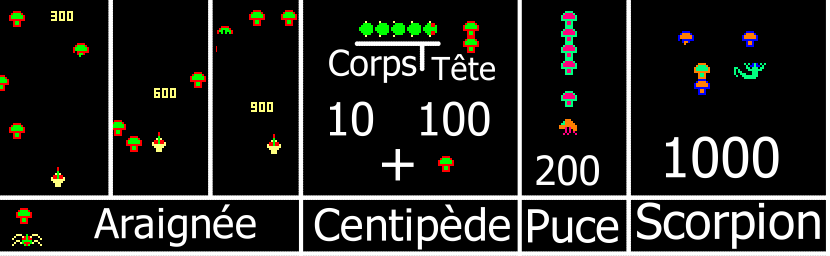
\includegraphics[width=\textwidth]{imgs/scoresCentipede.png}%
\label{fig:ScoresCenti}%
\end{figure}

Concernant les déplacements des ennemis, la puce et le scorpion se déplacent en ligne droite à leur vitesse, sans avoir d'obstacles. L'araignée remonte et descend aléatoirement et constamment mais se décalera toujours dans la même direction, mangeant les champignons sur son chemin. Enfin, quand la tête d'un centipède rencontre un champignon (collision) ou un bord de l'écran, il descend d'une ligne en ignorant les champignons et repart dans l'autre sens. Les autres segments suivront le même chemin. S'il a atteint la limite en bas, il détache sa queue qui devient alors une tête sur la dernière ligne, mais lui remonte.

%Si le joueur tue une partie du corps du centipède, celle-ci se transforme alors en champignon sur la position de sa mort et rapporte au joueur 10 points. Si le joueur touche la tête du centipède alors il gagne 100 points et transforme la tête du centipède en champignon. Si le joueur tue une araignée, celui-ci peut être récompensé en fonction des risques qu'il a pris pour tuer celle-ci. En effet, si le joueur tue l'araignée à une distance très proche de celle-ci alors il gagnera 900 points, à une distance moyenne il gagnera 600 points, et a une distance éloignée il gagnera 300 points. Le joueur peut également tuer les champignons qui possèdent chacun 4 points de vie. Il faut donc 4 tirs de la part du joueur afin de détruire un champignon. De plus les champignons ont une certaines visées stratégiques, car l'utilisateur peut les utiliser pour diriger le centipède là où il le veut et donc le tuer plus facilement. Le joueur peut tuer le scorpion qui rend les champignons vénéneux. Si le joueur y arrive alors il est récompensé par 1000 points. Le joueur peut aussi tuer une puce, ce qui lui rapporte 200 points. Cette puce apparaît seulement si il y a moins de 5 champignons dans la zone de déplacement du joueur. Elle apparaît aléatoirement en une position \emph{x} de la grille et  descend jusqu'en bas du tableau, en déposant des champignons aléatoirement en \emph{y}. De plus, un scorpion apparaît aléatoirement à partir d'un certain niveau et se déplace sur une ligne en rendant les champignons vénéneux. Dès lors si le centipède touche un des champignons vénéneux alors celui-ci descendra en ligne droite jusqu'à la zone du joueur. Ce qui rend le jeu encore plus difficile et ardu.
